%!TEX TS-program = pdflatex
\RequirePackage{fix-cm}
%\documentclass{article}
%\documentclass{svjour3}                     % onecolumn (standard format)
%\documentclass[smallcondensed]{svjour3}     % onecolumn (ditto)
\documentclass[smallextended]{svjour3}       % onecolumn (second format)
%\documentclass[twocolumn]{svjour3}          % twocolumn
\usepackage[utf8]{inputenc}


\usepackage[margin=1in]{geometry}
\usepackage[toc]{appendix}
\usepackage{natbib}

\usepackage{booktabs}
\usepackage{hyperref}


\makeatletter
\newcommand\footnoteref[1]{\protected@xdef\@thefnmark{\ref{#1}}\@footnotemark}
\makeatother


\usepackage{tikz}
\usetikzlibrary{arrows.meta,positioning,calc,shapes}
\usepackage[edges]{forest}
\definecolor{foldercolor}{RGB}{124,166,198}
\newcommand{\inputTikZ}[2]{%  
     \scalebox{#1}{\input{#2}}
}
\usepackage{varwidth}
\usepackage{pgfplots}

\usepackage{subfig}
\usepackage{epstopdf}
\usepackage{textcomp}


\usepackage[Symbol]{upgreek}

\graphicspath{.}

\title{Managing, storing, and sharing long-form recordings and their annotations}

\author{%
Lucas Gautheron \and Nicolas Rochat \and Alejandrina Cristia
}

\institute{
Laboratoire de Sciences Cognitives et de Psycholinguistique, Département d'Etudes cognitives, ENS, EHESS, CNRS, PSL University, Paris, France. 
\email{lucas.gautheron@gmail.com}
}

\journalname{Language Resources and Evaluation}

\date{}

\begin{document}

\maketitle

\abstract{
The technique of  long-form recordings via wearables is gaining momentum in different fields of research, notably linguistics and neurology. This technique, however, poses several technical challenges, some of which are amplified by the peculiarities of the data, including their sensitivity and their volume. In this paper, we begin by outlining key problems related to the management, storage, and sharing of the corpora  that emerge when using this technique. We continue by proposing a multi-component solution to these problems, specifically in the case of daylong recordings of children. As part of this solution, we release \emph{ChildProject}, a Python package for performing the operations typically required by such datasets and for evaluating the reliability of annotations using a number of measures commonly used in speech processing and linguistics. This package builds upon an annotation management system, which allows the importation of annotations from a wide range of existing formats, as well as upon data validation procedures, which assert the conformity of the data, or, alternatively, produce detailed and explicit error reports. Our proposal could be generalized to populations other than children and beyond linguistics. 
}

\keywords{daylong recordings, speech data management, data distribution, annotation evaluation, inter-rater reliability, reproducible research}


\section{Introduction}

Long-form recordings are those collected over extended periods of time, typically via a wearable. Although the technique was used with normotypical adults decades ago \citep{ear1,ear2}, it became widespread in the study of early childhood over the last decade since the publication of a seminal white paper by the LENA Foundation \citep{gilkerson2008power}. The LENA Foundation created a hardware-software combination that illuminated the potential of this technique for theoretical and applied purposes (e.g., \citealt{christakis2009audible,warlaumont2014social}). Fig. \ref{fig:data} summarizes which data are typically found in corpora of long-form recordings used for child language acquisition studies, while Fig. \ref{fig:annotations} illustrates annotations drawn from a public corpus.
More recently, long-form data is also being discussed in the context of neurological disorders (e.g., \citealt{riad2020vocal}). In this article, we define the unique space of difficulties surrounding long-form recordings, and introduce a set of packages that provides practical solutions, with a focus on child-centered recordings. Put briefly, we provide solutions that are compatible with a wide range of annotation and storage methods. These include a package that builds on existing standards to integrate functionalities for data processing and continuous validation, in addition to extant solutions allowing collaborative work and striking a balance between privacy on the one hand, reproducibility, findability, and long-term archiving on the other.  We end by discussing ways in which these solutions could be generalized to other populations.\footnote{In order to demonstrate how our proposal could foster reproducible research on long-form recordings of children, we have released the source code of the paper as well as the code used to build the figures in Section \ref{section:application}.}

\begin{figure}
    \centering
    \tikzset{%
  >={Latex[width=2mm,length=2mm]},
            base/.style = {rectangle, rounded corners, draw=black,
                           minimum width=4cm, minimum height=1cm,
                           text centered, font=\sffamily},
  recorder/.style = {base, fill=blue!30},
       meta/.style = {base, fill=red!30},
    annotator/.style = {base, fill=green!30},
          txt/.style = {font=\sffamily, text centered},
         title/.style = {txt, font=\sffamily\Large},
}

% Drawing part, node distance is 1.5 cm and every node
% is prefilled with white background
\begin{tikzpicture}[node distance=5cm,
    every node/.style={fill=white, font=\sffamily}, align=center]
  % Specification of nodes (position, etc.)
%   \node (lena) [recorder] {LENA recorder};
%   \node (babylogger) [recorder, right of=lena, xshift=5em] {BabyLogger};
%   \node (others) [recorder, right of=babylogger] {Other alternatives\\
%   \footnotesize{USB, Olympus...}};

%   \node (lena_software) [classifier, below of=lena, yshift = 5em] {LENA software\\
%   \footnotesize{Speaker type, Adult Word Count,}\\
%   \footnotesize{Child Vocalization Count, Conversational Turn Count}};
  
%   \node [txt, below of=lena_software, yshift=10em] {\large{LENA commercial environment}};

%   \node (vtc) [classifier, below of=babylogger, xshift=8em, yshift = 7em] {Voice Type Classifier (VTC)\\
%   \footnotesize {speech detection, speaker type classification}};
  
%   \node (alice) [classifier, below of=vtc, yshift = 8em] {Automatic LInguistic Unit Count Estimator (ALICE)\\
%   \footnotesize {phoneme, syllable and word counts}};


%   \node (seshat) [annotator, below of=lena_software, xshift=15em, yshift = 2em]  {Seshat\\
%   \footnotesize{web-based annotator}\\
%   \footnotesize{inter-rater reliability}};
   
%   \node (zooniverse) [annotator,right of=seshat]  {Zooniverse\\
%   \footnotesize{crowd-sourced classification tasks}};
   
%   \node (elan) [annotator, left of=seshat]  {ELAN\\
%   \footnotesize{annotation software}};
   
%   \node (das) [annotator, below of=elan, yshift = 10em]  {ACLEW DAS\\
%   \footnotesize{annotation scheme}};

%     \node (recorders) [title,right of=others] {Recording device};
%     \node (classifiers) [title,below of=recorders, yshift=3em] {Automatic annotation};
%     \node (annotators) [title,below of=classifiers, yshift=3em] {Manual annotation};


     
%   % Specification of lines between nodes specified above
%   % with aditional nodes for description 
%   \draw[->]             (lena) -- (lena_software);
%   \draw[->]             (vtc) -- (alice);
%   \draw[->]             (elan) -- (das);

% \draw [draw=black,dashed] ($(lena.north west) + (-2,0.5)$) rectangle ($(lena_software.south east) + (1,-1.5)$);

\node (media) [recorder] {
\Large \textbf{Media} \normalsize \\
($\sim 10^2$ to $10^4$ hours) \\
\framebox{
    {\begin{varwidth}{\linewidth}\begin{itemize}
        \item Audio (up to 24 hours \\ per recording)
        \item Video (up to 30 minutes \\ per recording)
        \item Accelerometer data (xyz)
        \item etc.
    \end{itemize}\end{varwidth}}
}};

\node (annotations) [annotator,shape=rectangle,draw,right of=media] {
\Large \textbf{Annotations} \normalsize \\
($\sim 10^5$ to $10^7$ segments)\\ \\
            \begin{tabular}{l r}
             \textbf{manual} & \textbf{automated}\\
              \multicolumn{2}{c}{who-speaks-when} \\
              \multicolumn{2}{c}{linguistic units} \\
              \multicolumn{2}{c}{vocal maturity} \\
               speech directedness &  \\
               transcriptions &  \\

            \end{tabular}
        };
        
\node (metadata) at ($(media)!0.5!(annotations)-(0,3)$) [meta,shape=rectangle,draw] {
\Large \textbf{Metadata} \normalsize \\ \\
            \framebox{
    {\begin{varwidth}{\linewidth}\begin{itemize}
        \item Recordings date and time, type of device, etc.
        \item Child date of birth, gender, normativity, etc.
        \item Socio-economic status, location, language(s), household size, etc.
        \item Questionnaires
    \end{itemize}\end{varwidth}}
}};
        


  \end{tikzpicture}
  

    \caption{\textbf{Data typically encountered in corpora of child-centered daylong recordings}. Media files (usually only audio recordings) are annotated by either humans or automated tools. Metadata often contain information about both the participant and their environment.}
    \label{fig:data}
\end{figure}
    
\begin{figure}
    \centering
    \includegraphics[width=0.8\linewidth]{Fig2.pdf}
    \caption{\label{fig:annotations}\textbf{Example of annotations derived from \cite{vandam-day}}. Annotator 1 positioned and labelled segments according to who was speaking and when, using the ELAN software \citep{wittenburg2006elan}. Annotator 2 transcribed speech using CHAT \citep{MacWhinney2000}. The LENA software \citep{gilkerson2008power} performed voice activation detection, speaker classification and count estimation.}
\end{figure}

\section{Problem space}\label{section:problemspace}

Management of scientific data is a long-standing issue which has been the subject of substantial progress in the recent years. For instance, FAIR principles (Findability, Accessibility, Interoperability, and Reusability; see \citealt{Wilkinson2016}) have been proposed to help improve the usefulness of data and data analysis pipelines. Similarly, databases implementing these practices have emerged, such as Dataverse \citep{dataverse} and Zenodo \citep{zenodo}. Long-form recordings cannot be treated in precisely the same way \citep{Cychosz2020}, and therefore require specific solutions. Below, we list some of the challenges that researchers are likely to face while employing long-form recordings in naturalistic environments.

\subsubsection*{The need for standards}

Extant datasets rely on a wide variety of metadata structures, file formats, and naming conventions. For instance, some data from long-form recordings have been archived publicly on Databrary (such as the ACLEW starter set \citealt{starter}) and HomeBank (including the VanDam Daylong corpus from \citealt{vandam-day}). Table \ref{table:datasets} shows some divergence across the two, which is simply the result of researchers working in parallel. As a result of this divergence, however, each lab finds itself re-inventing the wheel. For instance, the HomeBankCode organization\footnote{\url{https://github.com/homebankcode/}} contains at least 4 packages that do more or less the same operations, such as aggregating how much speech was produced in each recording, but implemented in different languages (MatLab,  R, perl, and Python). This divergence may also hide different operationalizations, rendering comparisons across labs fraught, effectively diminishing replicability.\footnote{\textit{Replicability} is typically defined as the effort to re-do a study with a new sample, whereas \textit{reproducibility} relates to re-doing the exact same analyses with the exact same data. Reproducibility is addressed in another section.} The variety of annotation formats (as illustrated in Fig. \ref{fig:annotations} for instance) has also led to duplication of efforts, as very similar tasks were implemented for one specific format and then later re-developed for another format.

Designing pipelines and analyses that are consistent across datasets requires standards for how the datasets are structured. Although this may represent an initial investment, such standards facilitate the pooling of research efforts, by allowing labs to benefit from code developed in other labs. Additionally, this field operates increasingly via collaborative cross-lab efforts. For instance, the ACLEW project\footnote{\url{https://sites.google.com/view/aclewdid/home}} involved nine principal investigators (PIs) from five different countries, who needed a substantive initial investment to agree on a standard organization for the six corpora used in the project \citep{soderstrom2021developing}. We expect even larger collaborations to emerge in the future, a move that would benefit from standardization, as exemplified by the community that emerged around CHILDES for short-form recordings \citep{macwhinney2000childes}. We show how building on the standards described in Section \ref{sec:format} allows our proposed Python package to accomplish a wide variety of tasks summarized in Section \ref{section:childproject}.

\begin{table}
\centering
\begin{tabular}{@{}lll@{}}
\toprule
                        & ACLEW starter  & VanDam \\ \midrule
\begin{tabular}[t]{@{}l@{}}Audios' scope\end{tabular}             & 5-minute clips & Full day       \\
\begin{tabular}[t]{@{}l@{}}Automated annotations'\\format\end{tabular}    & none         & LENA           \\
\begin{tabular}[t]{@{}l@{}}Human annotations'\\format\end{tabular} & .eaf           & .cha           \\
Human annotations' scope        & only clips     & Full day       \\
Metadata                & none           & excel \\ \bottomrule
\end{tabular}
\caption{\textbf{Divergences between the \cite{starter} and \cite{vandam-day} datasets}. Audios' scope indicates the size of the audio that has been archived: all recordings last for a full day, but for ACLEW starter, three five-minute clips were selected from each child. The automated annotations format indicates which software was used to annotate the audio automatically. Annotations' scope shows the scope of human annotation. Metadata indicates whether information about the children and recording were shared, and in what format.}
\label{table:datasets}
\end{table}


\subsubsection*{Keeping up with updates and contributions}

Datasets are not frozen. Rather, they are continuously enriched through annotations provided by humans or new algorithms. Human annotations may also undergo corrections as errors are discovered. The process of collecting the recordings may also require a certain amount of time, as they are progressively returned by the field workers or the participants themselves. In the case of longitudinal studies, supplementary audio data may accumulate over several years. Researchers should be able to keep track of these changes while also upgrading their analyses. Moreover, several collaborators may be brought to contribute work to the same dataset simultaneously. To take the example of ACLEW, PIs first annotated a random selection of 2-minute clips for 10 children in-house. They then exchanged some of these audio clips so that the annotators in another lab could re-annotate the same data, for the purposes of inter-rater reliability. This revealed divergences in definitions, and all datasets needed to be revised. Finally, a second sample of 2-minute clips with high levels of speech activity were annotated, and another process of reliability was performed. We suggest to solve these problems using DataLad \citep{datalad_paper}, an extension of git and one of the components of our proposed design, as explained in Section \ref{section:datalad}.

\subsubsection*{Performance and infrastructure}

Corpora of long-form recordings include large amounts of data, which raises a new set of challenges related to performance. 
Considering typical values for the bit depth and sampling rates of the recordings -- 16 bits and 16 kilohertz respectively -- yields a throughput of approximately three gigabytes per day of audio. Although there is a great deal of variation, past studies often involved at least 30 recording days (e.g., three days for each of ten children). The trend, however, is for datasets to be larger; for instance, last year, we collaborated in the collection of a single dataset, in which 200 children each contributed two recordings \citep{solomon-data}. Such datasets may exceed one terabyte. Moreover, these recordings can be associated with annotations spread across thousands of files. In the ACLEW example discussed above, there was one .eaf file per human annotator per each of four types of annotation (i.e., random, high speech, random reliability, high speech reliability). In addition, the full day was analyzed with between one and four automated routines. Thus, for each recording day there were 8 annotation files, leading to 6 corpora $\times$ 10 children $\times \ (4+4)$  annotations = 480 annotation files. Other researchers will use one annotation file per clip selected for annotation, which quickly adds up to thousands of files\footnote{For most ongoing research projects of which we are aware, there is no central annotation system; instead, annotators work in parallel on separate files. Some researchers may prefer to have the ``final'' version of the annotations in a merged format that represents the ``current best guess''. For transparency and clarity, however, such merged formats will emerge at a secondary stage, with a first stage represented by independent files including information about the independent listeners' judgments. Our package provides a solution that considers the current practice of working in parallel, but will adapt easily to alternative habits based on merged or collaborative formats.}.

Under such constraints, the storage, data delivery and data processing infrastructure plays a critical role. However, researchers' own infrastructure may be insufficient -- for instance, they may lack storage capacity, or GPU time --, and they may resort to outsourcing, e.g. using cloud providers. On the other hand, researchers that have access to their own cluster may favor that option instead of costly third-party services.
Ideally, a proper data management design should behave consistently regardless of a particular choice of infrastructure, provided the hardware meets some minimum standards. Users should not need to learn new techniques, procedures and software for each dataset they want to access.


Our proposal addresses the matter of data access performance by using DataLad (see Section \ref{section:datalad}), which supports a wide range of storage providers and is specifically designed to handle large files. Our Python package (Section \ref{section:childproject}) achieves scability by implementing parallelisation for most data processing operations. 



\subsubsection*{Privacy}

Long-form recordings are sensitive; they contain identifying and personal information about the participating family. In some cases, for instance if the family goes shopping and forgets to notify those around them, recordings could capture conversations which involve people who are unaware that they are being recorded. In addition, they may be subject to specific regulations, such as the European GDPR, the American HIPAA, and, depending on the place of collection and/or storage, laws on biometric data and incidental recording (which may vary across municipalities, states, and countries). For general ethical considerations, see \citet{Cychosz2020}. Here, we focus on privacy in the context of complying with FAIR guidelines when using long-form recordings.

However, although  long-form recordings are sensitive, many of the data types derived from them are not. With appropriate file-naming and meta-data practices, it is effectively possible to completely deidentify automated annotations (which at present never include automatic speech recognition). It is also often possible to deidentify human annotations, except when these involve transcribing what participants said, since participants will use personal names and reveal other personal details. Nonetheless, since this particular case involves a human doing the annotation, this human can be trained to modify the record (e.g., replace personal names with foils) and/or tag the annotation as sensitive and not to be openly shared. This is a practice called vetting, and it is one area in which the community working with long-form recordings has started to create standardized procedures, currently available from the HomeBank landing site (\url{homebank.talkbank.org}; e.g., \citealt{vandam2018vetting}).

Therefore, the ideal storing-and-sharing strategy should naturally enforce security and privacy safeguards by implementing access restrictions adapted to the level of confidentiality of the data. Data-access should be doable programmatically, and users should be able to download only the data that they need for their analysis. As argued in Sections \ref{section:datalad} and \ref{section:gin}, our proposal can solve this problem by enabling multi-tier data access.

\subsubsection*{Long-term availability}

The collection of long-form recordings requires a considerable level of investment to explain the technique to families and communities, to ensure a secure data management system, and, in the case of remote populations, to access the site. We have spent about 15,000 US\$ on a single round of data collection.\footnote{This grossly underestimates overall costs, because the best way to do any kind of field research is through maintaining strong bonds with the community and helping them in other ways throughout the year, not only during our visits (read more about ethical fieldwork on \citealt{broesch2020navigating}). A successful example for this is that of the UNM-UCSB Tsimane' Project (\url{http://tsimane.anth.ucsb.edu/}), which has been collaborating with the Tsimane' population since 2001. They are currently funded by a 5-year, 3-million US\$ NIH grant \url{https://reporter.nih.gov/project-details/9538306}. } These data are precious not only because of the investment that has gone into them, but also because they capture slices of life at a given point in time, which is particularly informative in the case of populations that are experiencing market integration or other forms of societal change -- which today is most or all populations. Moreover, some communities who are collaborating in such research speak languages that are minority languages in the local context, and thus at a potential risk for being lost in the future. The conservation of naturalistic speech samples of children's language acquisition throughout a normal day could be precious for fueling future efforts of language revitalization \citep{Nee2021}. It would therefore be particularly damaging to lose such data prematurely, from  financial,  scientific, and  human standpoints.

In addition, one advantage of long-form recordings over other observational methods such as parental reports is that they can be re-analyzed at later times to observe behaviors that had not been foreseen at the time of data collection. This implies that their interest partly lies in long-term re-usability.

Moreover, even state-of-the-art speech processing tools still perform poorly on long-form recordings, due to their intrinsic noisy nature \citep{casillas2019step}. As a result, taking full advantage of present data will necessitate new or improved computational models, which may take years to develop. For example, the DIHARD Challenge series has been running for three consecutive years, and documents the difficulty of making headway with complex audio data \citep{ryant2018first,ryant2019second,ryant2020third}. For instance, the best submission for speaker diarization in their meeting subcorpus achieved about 35\% Diarization Error Rate in 2018 and 2019, with improvements seen only in 2020, when the best system scored a 20\% Diarization Error Rate (Neville Ryant, personal communication, 2021-04-09). Other tasks are progressing much more slowly. For instance, the best performance in a classifier for deciding whether adult speech was addressed to the child or to an adult scored about 70\% correct in 2017 \citep{schuller2017interspeech} -- but nobody has been able to beat this record since. Recordings should therefore remain available for long periods of time -- potentially decades --, thus increasing the risk for data loss to occur at some point in their lifespan. For these reasons, the reliability of the storage design is critical, and redundancy is most certainly required. Likewise, persistent URLs may be needed in order to ensure the long-term accessibility of the datasets. These are key features of our proposal, as argued in sections \ref{section:datalad} and \ref{section:gin}.

\subsubsection*{Findability}

FAIR Principles include findability and accessibility. A crucial aspect of findability of datasets involves their being indexed in ways that potential re-users can discover them.  We would like to emphasize that findability of long-form recordings, especially those from under-represented populations, is of a peculiar importance. Indeed, although one of the many strengths of such recordings is that they can theoretically be sampled from any environment outside the lab, current corpora are still heavily biased in favor of WEIRD (Western, Educated, Industrialized, Rich, Democratic) populations: \cite{cychosz2021using} report that 81\% of samples (and 82\% of first authors) in papers included in systematic reviews of long-form recordings come from North America (with a further 12\% of samples, and 14\% of authors, based in Europe; see Figure 2). Not only more data should be collected from more diverse populations, but they should also be at least equally as findable and accessible in order to overcome the current representativeness bias. We would also like to stress again that the needs for Privacy and for Findability/Accessibility are not mutually exclusive. Although some of the data are of course sensitive, some of them could be made available to a broad audience without any harm to the privacy of the participants -- for instance, annotations that contain no transcription and parts of the metadata -- as discussed in the \textit{Privacy} section above.

Although we elaborate on it below, we want to already highlight HomeBank (\url{homebank.talkabank.org}; part of TalkBank, a recognized CLARIN Knowledge Centre) as one archiving option exists which is specific for long-form recordings, thus making any corpora hosted  there easily discoverable by other researchers using the technique. Also of relevance is Databrary (\url{databrary.org}), an archive specialized on child development, which can thus make the data visible to the developmental science community. However, the current standard practice  is archiving data in either one or another of these repositories, despite the fact that if a copy of the corpus were visible from one of these archives, the dataset would be overall more easily discovered. Additionally, it is uncertain whether these highly re-usable long-form recordings are visible to researchers who are more broadly interested in spoken corpora and/or naturalistic human behavior and/or other topics that could be studied in such data. In fact, one can conceive of a future in which the technique is used with people of different ages, in which case a system that allows users to discover other datasets based on relevant metadata would be ideal. For some research purposes (e.g., trying to stream overlapping voices and noise, technically referred to as "source separation") any recording may be useful, whereas for others (neurodegenerative disorders, early language acquisition) only some ages would. In any case, options exist to allow accessibility once a dataset is archived in one of those databases. We show how our proposed solution can be used to improve the findability of datasets in Sections \ref{section:datalad} and \ref{section:gin}.

\subsubsection*{Reproducibility}

Independent verification of results by a third party can be facilitated by improving the \emph{reproducibility} of the analyses, i.e. by providing third-parties with enough data and information to re-derive claimed results. This itself maybe be challenging for a number of reasons, including the variety of software requirements, unclear data dependencies, or insufficiently documented steps. Sharing data sets and analyses is more complex than delivering a collection of static files; all the information that is necessary in order to re-execute any intermediate step of the analysis should also be adequately conveyed. DataLad, which is one of the four components of our proposal, is specifically designed to increase reproducibility (see Section \ref{section:datalad}).

\subsubsection*{Current archiving options}

The field of child-centered long-form recordings has benefited from a purpose-built scientific archive from an early stage. HomeBank \cite{vandam2016homebank} builds on the same architecture as CHILDES \cite{MacWhinney2000} and other TalkBank corpora. Although this architecture served the purposes of the language-oriented community well for short recordings, there are numerous issues when using it for long-form recordings. To begin with, curators do not directly control their datasets' contents and structures, and if a curator wants to make a modification, they need to ask the HomeBank management team to make it for them. Similarly, other collaborators who spot errors cannot correct them directly, but again must request changes be made by the HomeBank management team.  Only one type of annotation is innately managed, and that is CHAT \cite{MacWhinney2000}, which is ideal for transcriptions of  recordings. However, transcriptions are of a lesser interest in child-centered long-form recordings because the amounts of audio they generate are such that humans would not be able to transcribe them to their full extent, and automatic transcription of such recordings -- which are very noisy -- is out of the reach of present models.

As briefly noted above, Databrary \url{databrary.org} also already hosts some long-form recording data. The aforementioned ACLEW project actually committed to archiving data there, rather than on HomeBank, because it allowed direct control and update (without needing to ask the HomeBank management).  As re-users, one of the most useful features of Databrary is the possibility to search the full archive for data pertaining to children of specific ages or origins. Using this archiving option led us to realize there were some limitations, including the fact that there is no Application Programming Interface (API) to retrieve the data programmatically at the time of writing, meaning that all updates need to be done via a graphical browser-based interface.

Additional options have been considered by researchers in the community, including OSF \footnote{\url{osf.io}}, and the Language Archive \footnote{\url{https://archive.mpi.nl/tla/}, which holds a CLARIN certificate B}. Detailing all their features is beyond the scope of the present paper, but some discussion can be found in \cite{casillas2019step}. As a way of explaining why we think they are insufficient solutions, OSF provides very limited storage capacities and requires no structure or metadata, thus does not solve problems of storage or standards. As for the Language Archive, it does not currently have an API for allowing updates of the data, nor automatic tests for its continued integrity.

Without denying their usefulness and importance, none of these archives provides perfect solutions to all of the problems we laid out above -- and notably, in our vision, researchers should not have to choose among them when archiving their data.   These limitations have brought us to envision a new strategy for sharing these datasets, which is detailed in Sections \ref{section:datalad} and \ref{section:gin}.

 \subsubsection*{Our proposal}
 
We propose a storing-and-sharing method designed to address the challenges outlined above simultaneously. It can be noted that these problems are, in many respects, similar to those faced by researchers in neuroimaging, a field which has long been confronting the need for reproducible analyses on large datasets of potentially sensitive data \citep{Poldrack2014}.
Their experience may, therefore, provide precious insight for linguists, psychologists, and developmental scientists engaging with the big-data approach of long-form recordings.
For instance, in the context of neuroimaging, \citet{Gorgolewski2016} have argued in favor of ``machine-readable metadata'', standard file structures and metadata, as well as consistency tests. Similarly, \citet{Eglen2017} have recommended the application of formatting standards, version control, and continuous testing. Before moving on, we would like to note that these concepts are all used in the key archiving options we evoked: HomeBank, Databrary, and the Language Archive all have defined metadata and file structures. However, they are {\it different} standards, which cannot be translated to each other, and which have not considered all the features that are relevant for long-form recordings, such as having multiple layers of annotations, with some based on sparse sampling. Additionally, the use of dataset versioning, automated consistency tests, and analyses based on subsumed datasets are less widespread in the language acquisition community. In the following, we will demonstrate how these practices have been implemented in our proposed design.
Albeit designed for child-centered long-form recordings, we believe our solution could be replicated across a wider range of datasets with constraints similar to those exposed above.

This solution relies on four main components, each of which is conceptually separable from the others: i) a standardized data format optimized for child-centered long-form recordings; ii) ChildProject, a Python package to perform basic operations on these datasets; iii) DataLad, ``a decentralized system for integrated discovery, management, and publication of digital objects of science'' \citep{hanke_defense_2021,datalad_paper} iv) GIN, a live archiving option for storage and distribution. Our choice for each one of these components can be revisited based on the needs of a project and/or as other options appear. Table \ref{table:components} summarizes which of these components helps address each of the challenges listed in Section \ref{section:problemspace}.

\begin{table*}[ht]
\centering
\begin{tabular}{@{}l|llll@{}}
\toprule
\textbf{Problem} &
  \begin{tabular}[t]{@{}l@{}}\textbf{ChildProject}\\(Section \ref{section:childproject})\end{tabular} &
  \begin{tabular}[t]{@{}l@{}}\textbf{DataLad}\\(Section \ref{section:datalad})\end{tabular} &
  \begin{tabular}[t]{@{}l@{}}\textbf{GIN}\\(Section \ref{section:gin})\end{tabular} \\ \midrule
The need for standards &
  \begin{tabular}[t]{@{}l@{}}documented standards;\\tests;\\conversion routines\end{tabular} &
   &
   \\ \midrule
\begin{tabular}[t]{@{}l@{}}Keeping up with updates\\ and contributions\end{tabular} &
   &
  \begin{tabular}[t]{@{}l@{}}version control\\(git)\end{tabular} &
  git repository host
   \\ \midrule
\begin{tabular}[t]{@{}l@{}}Performance\end{tabular} &
   parallelised processing &
  \begin{tabular}[t]{@{}l@{}}git-annex\\ (supports large files,\\ parallel download)\\\end{tabular} &
  \begin{tabular}[t]{@{}l@{}}git-annex compatible;\\ high storage capacity;\\ parallelised operations\end{tabular}
   \\ \midrule
Ensuring privacy & \begin{tabular}[t]{@{}l@{}}Optional metadata\\detection;\end{tabular}
   &
  \begin{tabular}[t]{@{}l@{}}private sub-datasets;\\ private remotes;\\
  path-based\\or metadata-based\\
  storage rules;\end{tabular} &
  \begin{tabular}[t]{@{}l@{}}Access Control Lists;\\SSH authentication\end{tabular}
   \\ \midrule
Long-term storage & \begin{tabular}[t]{@{}l@{}}tests\\(ensure integrity;\\
detect missing files)\end{tabular}
   &
  \begin{tabular}[t]{@{}l@{}}git; git-annex\\
  (remote synchronization,\\
  file availability and\\
  integrity checks,\\
  safe file deletion)\end{tabular} &
  DOI registration
  \\ \midrule
  Findability &
  \begin{tabular}[t]{@{}l@{}}rich and standardized\\ metadata\end{tabular} &
  \begin{tabular}[t]{@{}l@{}}metadata aggregation\\
  metadata search\end{tabular} &
  \begin{tabular}[t]{@{}l@{}}DOI registration;\\
  DataCite support\\
  repository search\end{tabular}
  \\ \midrule
Reproducibility &
   &
  \begin{tabular}[t]{@{}l@{}}run/rerun/container-run\\ functions\end{tabular} &

\end{tabular}
\caption{\textbf{\label{table:components}Contributions of each component of our proposed design in resolving the difficulties caused by long-form recordings} and laid out in Section \ref{section:problemspace}. ChildProject is a Python package designed to perform recurrent tasks on the datasets; DataLad is a Python package for the management of large, version-controlled datasets; GIN is a hosting provider dedicated to scientific data.}
\end{table*}

\section{Proposed solution}


\subsection{\label{sec:format}Dataset format}

\begin{figure}[ht]
    \centering
    \inputTikZ{0.8}{Fig4.tex}
    \caption{\textbf{Structure of a dataset}. Metadata, recordings and annotations each belong to their own folder. Raw annotations (i.e., the audio files as they have been collected, before post-processing) are separated from their post-processed counterparts (in this case: standardized and vetted recordings). Similarly, raw annotations (in this case, LENA's its annotations) are set apart from the corresponding CSV version.}
    \label{fig:tree}
\end{figure}

To begin with, we propose a set of proven standards which we use in the LAAC Team \url{https://lscp.dec.ens.fr/en/research/teams-lscp/language-acquisition-across-cultures} and which build on previous experience in several collaborative projects including ACLEW. It must be emphasized, however, that standards should be elaborated collaboratively by the community and that the following is merely a starting point.

Data that are part of the same collection effort are bundled together within one folder\footnote{We believe a reasonable unit of bundling is the collection effort, for instance a single field trip,  a full bout of data collection for a cross-sectional sample, or a set of recordings done more or less at the same time in a longitudinal sample. Given the possibilities of versioning, some users may decide they want to keep all data from a longitudinal sample in the same dataset, adding to it progressively over months and years, to avoid having duplicate children.csv files. That said, given DataLad's system of subdatasets (see Section \ref{section:datalad}), one can always define different datasets, each of which contains the recordings collected in subsequent time periods.}, preferably a DataLad dataset (see Section \ref{section:datalad}). Datasets are packaged according to the structure given in fig. \ref{fig:tree}. The \path{metadata} folder contains at least three dataframes in CSV format: (i) \path{children.csv} contains information about the participants, such as their age or the language(s) they speak. (ii) \path{recordings.csv} contains the metadata for each recording, such as when the recording started, which device was used, or its relative path in the dataset. (iii) \path{annotations.csv} contains information concerning the annotations provided in the dataset, how they were produced, or which range they cover, etc. Metadata that are sensitive (e.g. names) and which should only be shared with a limited audience can be placed into \path{metadata/recordings/} or \path{metadata/children/}; the package will automatically detect their presence and import them if they are available.

The dataframes are standardized according to guidelines which set conventional names for the columns and the range of allowed values. The guidelines are enforced through tests which print all the errors and inconsistencies in a dataset implemented in the ChildProject package introduced below.

The \path{recordings} folder contains two subfolders: \path{raw}, which stores the recordings as delivered by the experimenters, and \path{converted}, which contains processed copies of the recordings. All the audio files in \path{recordings/raw} are indexed in the recordings dataframe. Thus, there is no need for naming conventions for the audio files themselves, and maintainers can decide how they want to organize them.

The \path{annotations} folder contains all sets of annotations. Each set itself consists of a folder containing two subfolders: i) \path{raw}, which stores the output of the annotation pipelines and ii) \path{converted}, which stores the annotations after being converted to a standardized CSV format and indexed into \path{metadata/annotations.csv}. A set of annotations can contain an unlimited amount of subsets, with any amount of recursions. For instance, a set of human-produced annotations could include one subset per annotator. Recursion facilitates the inheritance of access permissions, as explained in Section \ref{section:datalad}.


\subsection{ChildProject}\label{section:childproject}

The ChildProject package is a Python 3.6+ package that performs common operations on a dataset of child-centered recordings. It can be used from the command-line or by importing the modules from within Python. It should be noted that the Python API stores metadata and annotations as Pandas dataframes \citep{Pandas-software,Pandas-paper}. As a result of relying on such a widely used scientific library, it is not necessary to learn new data types in order to use this package. Moreover, most operations are thus naturally vectorized, which contributes to better performance.

Assuming the target datasets are packaged according to the standards summarized in Section \ref{sec:format}, the package supports the functions listed below.

\subsubsection*{Listing errors and inconsistencies in a dataset}

We provide a validation script that returns a detailed reporting of all the errors found within a dataset, such as violations of the formatting guidelines or missing files. Tests help enforce the standards that allow the commensurability of the datasets while guaranteeing the integrity and coherence of the data.

\subsubsection*{Converting and indexing annotations}\label{section:annotations}

Fig. \ref{fig:annotations} shows that, whatever their format, annotations are always conceptually segments delimited by an onset and an offset timestamps, to which are attached a number of properties such as a speaker's identity or a transcription. Therefore, annotations can almost always be represented as Pandas dataframes, with one row per segment and one column per property.

Taking advantage of this, the package converts input annotations to standardized, wide-table CSV dataframes\footnote{\url{https://childproject.readthedocs.io/en/paper/annotations.html}}. The columns in these wide-table formats have been determined based on previous work, and are largely specific to the goal of studying infants' language environment and production. However, users can introduce custom columns if required.

Annotations are indexed into a unique CSV dataframe which stores their location in the dataset, the set of annotations they belong to, and the recording and time interval they cover. The index, therefore, allows an easy retrieval of all the annotations that cover any given segment of audio, regardless of their original format and the naming conventions that were used. The system interfaces well with extant annotation standards. Currently, ChildProject supports: LENA annotations in .its \citep{xu2008lenatm}; ELAN annotations following the ACLEW DAS template  (\citealt{Casillas2017}, imported using Pympi: \citealt{pympi-1.70}); CHAT annotations \citep{MacWhinney2000}; as well as rttm files outputted by ACLEW tools, namely the Voice Type Classifier (VTC) by \citet{lavechin2020opensource}, the Automatic Linguistic Unit Count Estimator (ALICE) by \citet{rasanen2020}, and the VoCalisation Maturity Network (VCMNet) by \citet{AlFutaisi2019}. Users can also adapt routines for file types or conventions that vary. For instance, users can adapt the ELAN import developed for the ACLEW DAS template for their own template (e.g., \url{https://github.com/LAAC-LSCP/ChildProject/discussions/204}); and examples are also provided for Praat's .TextGrid files \citep{boersma2006praat}. The package also supports custom, user-defined conversion routines.

Relying on the annotations index, the package can also calculate the intersection of the portions of audio covered by several annotators and align their annotations. This is useful when annotations from different annotators need to be combined (in order to retain the majority choice for instance) or compared (e.g., for reliability evaluations).

\subsubsection*{Choosing audio samples of the recordings to be annotated}\label{section:choosing}

As noted in the Introduction, recordings are too extensive to be manually annotated in their entirety. We and colleagues have typically annotated manually clips of 0.5-5 minutes in length, and the way these clips are extracted and annotated varies (as illustrated in Table \ref{table:datasets}).

The package allows the use of predefined or custom sampling algorithms\footnote{\url{https://childproject.readthedocs.io/en/paper/samplers.html}}. Samples' timestamps are exported to CSV dataframes. In order to keep track of the sample generating process, input parameters are simultaneously saved into a YAML file. Predefined samplers include a periodic sampler, a sampler targeting specific speakers' vocalizations, a sampler targeting regions of high-volubility according to input annotations, and a more agnostic sampler targeting high-energy regions. In all cases, the user can define the number of regions and their duration, as well as the context that may be inspected by human annotators. These options cover all documented sampling strategies. Evaluations of the performance of some of these samplers can be found in \citep[Chapter 15, ``Human annotation'']{exelang-book}.

\subsubsection*{Generating ELAN files ready to be annotated}

Although there was some variability in terms of the program used for human annotation, the field has now by and large settled on ELAN \citep{wittenburg2006elan}. ELAN employs xml files with a hierarchical structure which are both customizable and flexible. The ChildProject can be used to generate .eaf files which can be annotated with the ELAN software\footnote{\url{https://childproject.readthedocs.io/en/paper/elan.html}} based on samples of the recordings drawn using the package, as described in Section \ref{section:choosing}.

\subsubsection*{Extracting and uploading audio samples to Zooniverse}

The crowd-sourcing platform Zooniverse \citep{zooniverse} has been extensively employed in both natural \citep{gravityspy} and social sciences. More recently, researchers have been investigating its potential to classify samples of audio extracted from long-form recordings of children and the results have been encouraging  \citep{semenzin2020a,semenzin2020b}. We provide tools interfacing with Zooniverse's API for preparing and uploading audio samples to the platform and for retrieving the results, while protecting the privacy of the participants\footnote{\url{https://childproject.readthedocs.io/en/paper/zooniverse.html}}. A step-by-step tutorial including re-usable code is also provided \citep{zooniverse_example}.

\subsubsection*{Audio processing}

ChildProject allows the batch-conversion of the recordings to any target audio format (thanks to \citealt{ffmpeg})\footnote{\url{https://childproject.readthedocs.io/en/paper/processors.html}}.

The package also implements a ``vetting" \citep{vandam2018vetting,Cychosz2020} pipeline, which mutes segments of the recordings previously annotated by humans as confidential while preserving the duration of the audio files. After being processed, the recordings can safely be shared with other researchers or annotators.

Another pipeline allows to perform filtering or linear combinations of audio channels for multi-channel recordings such as those produced with the BabyLogger\footnote{\url{https://docs.babycloudlab.com/}}; if necessary, users can easily design custom audio converters suiting more specific needs.

\subsubsection*{Metrics extraction}

The package includes a pipeline to extract metrics that are commonly used in this research area -- such as the speech rates of each speaker -- by aggregating annotations at the desired level, e.g. per recording or per child\footnote{\url{https://childproject.readthedocs.io/en/paper/metrics.html}}. Metrics can also be aggregated depending on the time of the day, where the width of the time bins is chosen by the user.

\subsubsection*{Other functionalities}

The package offers additional functions such as a pipeline that strips LENA's annotations from data that could be used to identify the participants, built upon previous code by \citet{eaf-anonymizer-original}.

Notably, the package facilitates the computation of a number of typical measures of annotations reliability and accuracy, as demonstrated in Section \ref{section:application}.

\subsubsection*{User empowerment}

The present effort is led by one research team, and thus with personnel and funding that is not permanent. We therefore have done our best to provide information to help the community adopt and maintain this code in the future. Extensive documentation is provided on \url{https://childproject.readthedocs.io}, including detailed tutorials. The code is accessible on GitHub.com.


\subsection{DataLad}\label{section:datalad}

\begin{figure}[htb]
\centering
\begin{minipage}{.5\linewidth}
\centering
\subfloat[]{\label{datalad:a}\resizebox{!}{0.70\linewidth}{\large% GNUPLOT: LaTeX picture with Postscript
\begingroup
  \makeatletter
  \providecommand\color[2][]{%
    \GenericError{(gnuplot) \space\space\space\@spaces}{%
      Package color not loaded in conjunction with
      terminal option `colourtext'%
    }{See the gnuplot documentation for explanation.%
    }{Either use 'blacktext' in gnuplot or load the package
      color.sty in LaTeX.}%
    \renewcommand\color[2][]{}%
  }%
  \providecommand\includegraphics[2][]{%
    \GenericError{(gnuplot) \space\space\space\@spaces}{%
      Package graphicx or graphics not loaded%
    }{See the gnuplot documentation for explanation.%
    }{The gnuplot epslatex terminal needs graphicx.sty or graphics.sty.}%
    \renewcommand\includegraphics[2][]{}%
  }%
  \providecommand\rotatebox[2]{#2}%
  \@ifundefined{ifGPcolor}{%
    \newif\ifGPcolor
    \GPcolorfalse
  }{}%
  \@ifundefined{ifGPblacktext}{%
    \newif\ifGPblacktext
    \GPblacktexttrue
  }{}%
  % define a \g@addto@macro without @ in the name:
  \let\gplgaddtomacro\g@addto@macro
  % define empty templates for all commands taking text:
  \gdef\gplbacktext{}%
  \gdef\gplfronttext{}%
  \makeatother
  \ifGPblacktext
    % no textcolor at all
    \def\colorrgb#1{}%
    \def\colorgray#1{}%
  \else
    % gray or color?
    \ifGPcolor
      \def\colorrgb#1{\color[rgb]{#1}}%
      \def\colorgray#1{\color[gray]{#1}}%
      \expandafter\def\csname LTw\endcsname{\color{white}}%
      \expandafter\def\csname LTb\endcsname{\color{black}}%
      \expandafter\def\csname LTa\endcsname{\color{black}}%
      \expandafter\def\csname LT0\endcsname{\color[rgb]{1,0,0}}%
      \expandafter\def\csname LT1\endcsname{\color[rgb]{0,1,0}}%
      \expandafter\def\csname LT2\endcsname{\color[rgb]{0,0,1}}%
      \expandafter\def\csname LT3\endcsname{\color[rgb]{1,0,1}}%
      \expandafter\def\csname LT4\endcsname{\color[rgb]{0,1,1}}%
      \expandafter\def\csname LT5\endcsname{\color[rgb]{1,1,0}}%
      \expandafter\def\csname LT6\endcsname{\color[rgb]{0,0,0}}%
      \expandafter\def\csname LT7\endcsname{\color[rgb]{1,0.3,0}}%
      \expandafter\def\csname LT8\endcsname{\color[rgb]{0.5,0.5,0.5}}%
    \else
      % gray
      \def\colorrgb#1{\color{black}}%
      \def\colorgray#1{\color[gray]{#1}}%
      \expandafter\def\csname LTw\endcsname{\color{white}}%
      \expandafter\def\csname LTb\endcsname{\color{black}}%
      \expandafter\def\csname LTa\endcsname{\color{black}}%
      \expandafter\def\csname LT0\endcsname{\color{black}}%
      \expandafter\def\csname LT1\endcsname{\color{black}}%
      \expandafter\def\csname LT2\endcsname{\color{black}}%
      \expandafter\def\csname LT3\endcsname{\color{black}}%
      \expandafter\def\csname LT4\endcsname{\color{black}}%
      \expandafter\def\csname LT5\endcsname{\color{black}}%
      \expandafter\def\csname LT6\endcsname{\color{black}}%
      \expandafter\def\csname LT7\endcsname{\color{black}}%
      \expandafter\def\csname LT8\endcsname{\color{black}}%
    \fi
  \fi
    \setlength{\unitlength}{0.0500bp}%
    \ifx\gptboxheight\undefined%
      \newlength{\gptboxheight}%
      \newlength{\gptboxwidth}%
      \newsavebox{\gptboxtext}%
    \fi%
    \setlength{\fboxrule}{0.5pt}%
    \setlength{\fboxsep}{1pt}%
\begin{picture}(7200.00,5040.00)%
    \gplgaddtomacro\gplbacktext{%
      \csname LTb\endcsname%%
      \put(682,440){\makebox(0,0)[r]{\strut{}$0$}}%
      \put(682,1170){\makebox(0,0)[r]{\strut{}$10$}}%
      \put(682,1900){\makebox(0,0)[r]{\strut{}$20$}}%
      \put(682,2630){\makebox(0,0)[r]{\strut{}$30$}}%
      \put(682,3359){\makebox(0,0)[r]{\strut{}$40$}}%
      \put(682,4089){\makebox(0,0)[r]{\strut{}$50$}}%
      \put(682,4819){\makebox(0,0)[r]{\strut{}$60$}}%
      \put(814,220){\makebox(0,0){\strut{}01/15}}%
      \put(1811,220){\makebox(0,0){\strut{}01/16}}%
      \put(2812,220){\makebox(0,0){\strut{}01/17}}%
      \put(3809,220){\makebox(0,0){\strut{}01/18}}%
      \put(4804,220){\makebox(0,0){\strut{}01/19}}%
      \put(5801,220){\makebox(0,0){\strut{}01/20}}%
      \put(6802,220){\makebox(0,0){\strut{}01/21}}%
    }%
    \gplgaddtomacro\gplfronttext{%
      \csname LTb\endcsname%%
      \put(209,2629){\rotatebox{-270}{\makebox(0,0){\strut{}DataLad versions released}}}%
    }%
    \gplbacktext
    \put(0,0){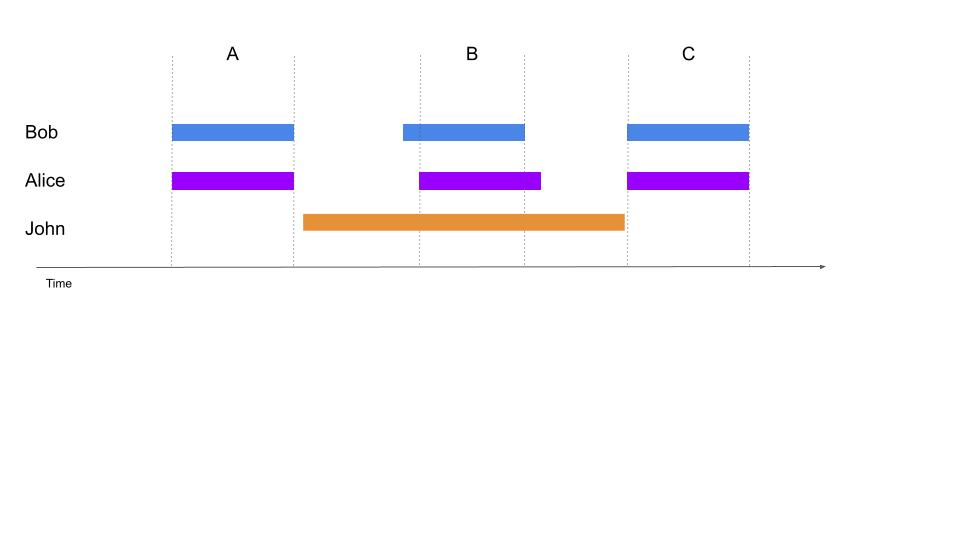
\includegraphics[width={360.00bp},height={252.00bp}]{Fig3a}}%
    \gplfronttext
  \end{picture}%
\endgroup
\normalsize}}
\end{minipage}%
\begin{minipage}{.5\linewidth}
\centering
\subfloat[]{\label{datalad:b}\resizebox{!}{0.70\linewidth}{\large% GNUPLOT: LaTeX picture with Postscript
\begingroup
  \makeatletter
  \providecommand\color[2][]{%
    \GenericError{(gnuplot) \space\space\space\@spaces}{%
      Package color not loaded in conjunction with
      terminal option `colourtext'%
    }{See the gnuplot documentation for explanation.%
    }{Either use 'blacktext' in gnuplot or load the package
      color.sty in LaTeX.}%
    \renewcommand\color[2][]{}%
  }%
  \providecommand\includegraphics[2][]{%
    \GenericError{(gnuplot) \space\space\space\@spaces}{%
      Package graphicx or graphics not loaded%
    }{See the gnuplot documentation for explanation.%
    }{The gnuplot epslatex terminal needs graphicx.sty or graphics.sty.}%
    \renewcommand\includegraphics[2][]{}%
  }%
  \providecommand\rotatebox[2]{#2}%
  \@ifundefined{ifGPcolor}{%
    \newif\ifGPcolor
    \GPcolorfalse
  }{}%
  \@ifundefined{ifGPblacktext}{%
    \newif\ifGPblacktext
    \GPblacktexttrue
  }{}%
  % define a \g@addto@macro without @ in the name:
  \let\gplgaddtomacro\g@addto@macro
  % define empty templates for all commands taking text:
  \gdef\gplbacktext{}%
  \gdef\gplfronttext{}%
  \makeatother
  \ifGPblacktext
    % no textcolor at all
    \def\colorrgb#1{}%
    \def\colorgray#1{}%
  \else
    % gray or color?
    \ifGPcolor
      \def\colorrgb#1{\color[rgb]{#1}}%
      \def\colorgray#1{\color[gray]{#1}}%
      \expandafter\def\csname LTw\endcsname{\color{white}}%
      \expandafter\def\csname LTb\endcsname{\color{black}}%
      \expandafter\def\csname LTa\endcsname{\color{black}}%
      \expandafter\def\csname LT0\endcsname{\color[rgb]{1,0,0}}%
      \expandafter\def\csname LT1\endcsname{\color[rgb]{0,1,0}}%
      \expandafter\def\csname LT2\endcsname{\color[rgb]{0,0,1}}%
      \expandafter\def\csname LT3\endcsname{\color[rgb]{1,0,1}}%
      \expandafter\def\csname LT4\endcsname{\color[rgb]{0,1,1}}%
      \expandafter\def\csname LT5\endcsname{\color[rgb]{1,1,0}}%
      \expandafter\def\csname LT6\endcsname{\color[rgb]{0,0,0}}%
      \expandafter\def\csname LT7\endcsname{\color[rgb]{1,0.3,0}}%
      \expandafter\def\csname LT8\endcsname{\color[rgb]{0.5,0.5,0.5}}%
    \else
      % gray
      \def\colorrgb#1{\color{black}}%
      \def\colorgray#1{\color[gray]{#1}}%
      \expandafter\def\csname LTw\endcsname{\color{white}}%
      \expandafter\def\csname LTb\endcsname{\color{black}}%
      \expandafter\def\csname LTa\endcsname{\color{black}}%
      \expandafter\def\csname LT0\endcsname{\color{black}}%
      \expandafter\def\csname LT1\endcsname{\color{black}}%
      \expandafter\def\csname LT2\endcsname{\color{black}}%
      \expandafter\def\csname LT3\endcsname{\color{black}}%
      \expandafter\def\csname LT4\endcsname{\color{black}}%
      \expandafter\def\csname LT5\endcsname{\color{black}}%
      \expandafter\def\csname LT6\endcsname{\color{black}}%
      \expandafter\def\csname LT7\endcsname{\color{black}}%
      \expandafter\def\csname LT8\endcsname{\color{black}}%
    \fi
  \fi
    \setlength{\unitlength}{0.0500bp}%
    \ifx\gptboxheight\undefined%
      \newlength{\gptboxheight}%
      \newlength{\gptboxwidth}%
      \newsavebox{\gptboxtext}%
    \fi%
    \setlength{\fboxrule}{0.5pt}%
    \setlength{\fboxsep}{1pt}%
\begin{picture}(7200.00,5040.00)%
    \gplgaddtomacro\gplbacktext{%
      \csname LTb\endcsname%%
      \put(946,374){\makebox(0,0)[r]{\strut{}$0$}}%
      \put(946,1009){\makebox(0,0)[r]{\strut{}$0.05$}}%
      \put(946,1644){\makebox(0,0)[r]{\strut{}$0.1$}}%
      \put(946,2279){\makebox(0,0)[r]{\strut{}$0.15$}}%
      \put(946,2914){\makebox(0,0)[r]{\strut{}$0.2$}}%
      \put(946,3549){\makebox(0,0)[r]{\strut{}$0.25$}}%
      \put(946,4184){\makebox(0,0)[r]{\strut{}$0.3$}}%
      \put(946,4819){\makebox(0,0)[r]{\strut{}$0.35$}}%
    }%
    \gplgaddtomacro\gplfronttext{%
      \csname LTb\endcsname%%
      \put(209,2596){\rotatebox{-270}{\makebox(0,0){\strut{}Fraction of commits}}}%
      \put(3940,154){\makebox(0,0){\strut{}Top contributors}}%
    }%
    \gplbacktext
    \put(0,0){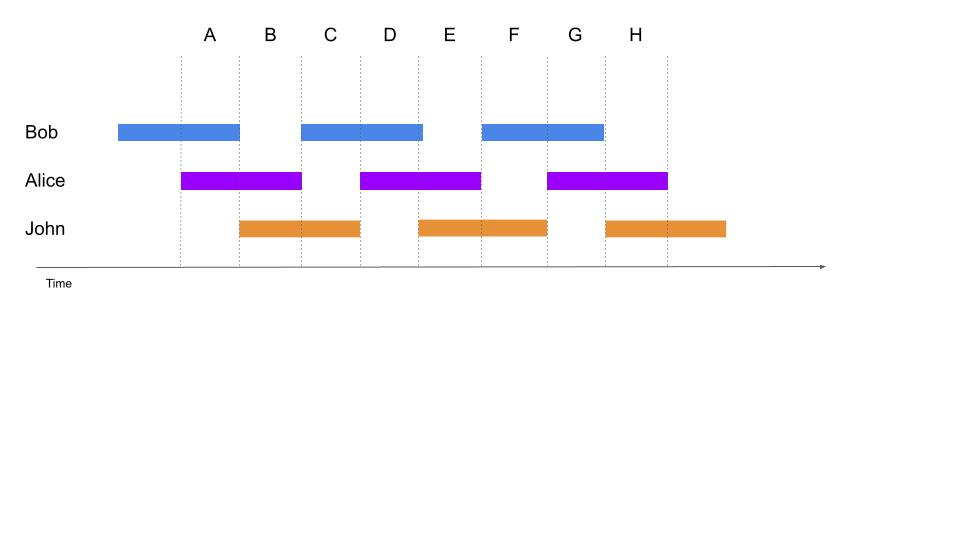
\includegraphics[width={360.00bp},height={252.00bp}]{Fig3b}}%
    \gplfronttext
  \end{picture}%
\endgroup
\normalsize}}
\end{minipage}\par\medskip


\caption{\label{fig:datalad}\textbf{DataLad development activity}. (a) Amount of versions published across time. More than 50 versions have been released since 2015-01-01, at a steady pace. (b) Share of git commits held by top contributors in the last year (2020). At least three developers have contributed substantially, each of them being responsible for about 30\% of the commits.}

\end{figure}

The combination of standards and the ChildProject package allows us to solve some of the problems laid out in the Introduction, but they do not directly provide solutions to the problems of data sharing and collaborative work. DataLad, however, has been specifically designed to address such needs.

DataLad \citep{datalad_paper} was initially developed by researchers from the computational neuroscience community for the sharing of neuroimaging datasets. It has been under active development at a steady pace for at least six years (fig. \ref{datalad:a}). It is co-funded by the United States NSF and the German Federal Ministry of Education and Research and has several major code developers (fig. \ref{datalad:b}).% thereby lowering its bus-factor\footnote{\url{https://en.wikipedia.org/wiki/Bus_factor}} :D.

DataLad relies on git-annex, a software designed to manage large files with git. Over the years, git has rapidly overcome competitors such as Subversion, and it has been popularized by platforms such as GitLab and GitHub. However, git does not natively handle large binary files, our recordings included. Git-annex circumvents this issue by only versioning pointers to the large files. The actual content of the files is stored in an ``annex''. Annexes can be stored remotely on a variety of supports, including Amazon Glacier, Amazon S3, Backblaze B2, Box.com, Dropbox, FTP/SFTP, Google Cloud Storage, Google Drive, Internet Archive via S3, Microsoft Azure Blob Storage, Microsoft OneDrive, OpenDrive, OwnCloud, SkyDrive, Usenet, and Yandex Disk.

A DataLad dataset is, essentially, a git repository with an annex. As such, it naturally allows version control, easy collaboration with many contributors, and continuous testing. Furthermore, its use is intuitive to git users.

In using git-annex, DataLad enables users to download only the files that they need, without needing to fetch the whole dataset.

DataLad improves upon git-annex by adding a number of functionalities. One of them, dataset nesting, is built upon git submodules. A DataLad dataset can include sub-datasets, with as many levels of recursion as needed. This provides a natural solution to the question of how to document analyses, as an analysis repository can have the dataset on which it depends embedded as a subdataset. It also provides a good solution for the issue of different levels of data containing more or less identifying information, via the possibility of restricting permissions to different levels of the hierarchy.

Like git, DataLad is a decentralized system, meaning that data can be stored and replicated across several ``remotes''. DataLad authors have argued in favor of decentralized research data management, as it simplifies infrastructure migrations, and helps improve the scalibility of the data storage and distribution design \cite{decentralization_hanke}. Additionally, decentralization is notably useful in that it facilitates redundancy; files can be pushed simultaneously to several storage supports (e.g.: an external hard-drive, a cloud provider), thereby reducing the risk of data loss. In addition to that, by default, DataLad refuses to delete a local copy of a large file unless a certain amount of remotes -- which can be configured by the user -- still own a copy the data. Of course, a user may still remove every copy of a file by using forced deletion or by setting the minimum amount of copies to zero.

Many of the \emph{remotes} supported by DataLad require user-authentication, thus allowing for fine-grained access permissions management, such as Access-Control Lists (ACL). There are at least two ways to implement multiple levels of access within a dataset. One involves using sub-datasets with stricter access requirements. It is also possible to store data across several git-annex remotes with varying access permissions, depending on their sensitivity. Path-based pattern matching rules may be configured in order to automatically select which remote the files should be pushed to. More flexible selection rules can be implemented using git-annex metadata, which allows to label files with \texttt{key=value} pairs. For instance, one could tag confidential files as \texttt{confidential=yes} and exclude these from certain remotes (blacklist). Alternatively, some files could be pushed to a certain remote provided they are labelled \texttt{public=yes} (whitelist).

DataLad's metadata\footnote{\url{http://docs.datalad.org/en/stable/metadata.html}} system can extract and aggregate information describing the contents of a collection of datasets. A search function then allows the discovery of datasets based on these metadata. We have developed a DataLad extension to extract meaningful metadata from datasets into DataLad's metadata system \citep{datalad_extension}. This allows, for instance, to search for datasets containing a given language. Moreover, DataLad's metadata can natively incorporate DataCite \citep{brase2009datacite} descriptions into its own metadata.

DataLad may link data and software dependencies associated to a script as it is run. These scripts can later be re-executed by others, and the dependencies will automatically be downloaded. This way, DataLad can keep track of how each intermediate file was generated, thus simplifying the reproducibility of analyses. DataLad's handbook provides a tutorial to create a fully reproducible paper \citep[Chapter~22]{datalad_handbook}, and a template is available on GitHub \citep{reproducible_paper}. The present paper has been built upon this template, and its source is available on GIN\footnote{\url{https://gin.g-node.org/LAAC-LSCP/managing-storing-sharing-paper}}.

DataLad is domain-agnostic, which makes it suitable for maturing techniques such as language acquisition studies based on long-form recordings. The open-access data of the WU-Minn Human Connectome Project \citep{pub.1022076283}, totalling 80 terabytes to date, have been made available through DataLad \footnote{\label{note:hcp}\url{https://github.com/datalad-datasets/human-connectome-project-openaccess}}.


\subsection{Storage and distribution}\label{section:gin}

DataLad does not provide, by itself, the infrastructure to share data. However, it allows maintainers to publish their content to a wide range of \href{https://git-annex.branchable.com/special_remotes/}{platforms}. One can therefore implement different strategies for the storage and distribution of the data using any combination of these providers, depending on the constraints.

Table \ref{table:providers} sums up the most relevant characteristics of a few providers that are appropriate for our research, although many more could be considered. Datasets can only be cloned from providers that support git, and the large files can only be stored on those that support git-annex. Platforms that only support the former, such as GitHub, should therefore be used in tandem with providers that support the latter, like Amazon S3.

Among criteria of special interest are: the provider's ability to handle complex permissions; how much data it can accept; its ability to assign permanent URLs and identifiers to the datasets; and of course, whether it complies with the legislation regarding privacy. For our purposes, Table \ref{table:providers} suggests GIN is the best option, handling well large files, with highly customizable permissions, and Git-based version control and access (see Appendix \ref{appendix:gin} for a practical use-case of GIN). That said, private projects are limited in space, although at the time of writing this limit can be raised by contributions to the GIN administrators. Moreover, there is no long-term guarantee that GIN will keep operating as it currently does. However, GIN's software is open-source, enabling users to run their own instance, where they could move their data to at any time -- which is very straightforward with DataLad. The next best option may be S3, and some users may prefer S3 when they do not have access to a local cluster, since S3 allows both easy storage and processing. 

To render comparison of options easier, detailed examples of storage designs taken from real datasets are listed in Appendix \ref{appendix:examples}. Scripts to implement these strategies can be found on our GitHub and OSF \citep{datalad_procedures}. We also provide a tutorial based on a public corpus \citep{vandam-day} to convert existing data to our standards and then publish it with DataLad\footnote{\url{https://childproject.readthedocs.io/en/paper/vandam.html}}.
We would like to emphasize that the flexibility of DataLad makes it very easy to migrate from one architecture to another. The underlying infrastructure may change, with little to no impact on the users, and little efforts from the maintainers.

In any case, we strongly recommend users to bear in mind that redundancy is important to make sure data are not lost, so a backup sibling may be hosted in an additional site (e.g., in a computer on campus in addition to the cloud-based version). 

For instance, \citet{Perkel_2019} suggests several practices regarding backups, including automated backups, privacy safe-guarding, regular tests, and offline backups. Table \ref{table:backups} may orient the reader towards the functionalities of DataLad (and git-annex) which can be used to achieve these goals.

\begin{table*}[ht]

\begin{minipage}{\columnwidth}%
\centering
\renewcommand\footnoterule{ \kern -1ex}
\renewcommand{\thempfootnote}{\alph{mpfootnote}}

\begin{tabular}{@{}lllllll@{}}
\toprule
\multicolumn{1}{c}{\textbf{Provider}} & \multicolumn{1}{c}{\textbf{Git}\footnote{The provider can store the git history and provide an URL from which the dataset can be installed.}} & \multicolumn{1}{c}{\textbf{Large files}\footnote{The provider handles git-annex large files.}} & \multicolumn{1}{c}{\textbf{Authentication}} & \multicolumn{1}{c}{\textbf{Permissions}} & \multicolumn{1}{c}{\textbf{Quota}} &
\multicolumn{1}{c}{\textbf{\begin{tabular}[t]{@{}l@{}}DOI\\registration\end{tabular}}} \\ \midrule
\midrule
SSH server                            & Yes                              & Yes                                      & SSH                                         & Unix                                     & Self-hosted & No                                 \\
GIN                                   & Yes                              & Yes                                      & HTTPS or SSH                                            & ACL                                      & \footnote{\label{contact}Contact the administrators} 
 & Yes\footnoteref{contact}\\
GitHub                                & Yes                              & No                                       & HTTPS or SSH                                & ACL                                      & --  & No                                \\
GitLab                                & Yes                              & No                                       & HTTPS or SSH                                & ACL                                      & --  & No                                \\

Nextcloud                             & No                               & Yes                                      &                                             & ACL                                      & Self-hosted & No                                 \\
Amazon S3                             & No                               & Yes                                      & API key+secret                              & IAM                                      & Unlimited & No                                  \\
OSF                                   & Yes\footnote{\label{osf}With limitations (see \url{http://docs.datalad.org/projects/osf/en/latest/intro.html})}                             & Yes\footnoteref{osf}                                     & Token                                       & ACL                                      & \footnote{5 GB for private projects, 50 GB for publics projects}  & Yes                              \\                                 
\end{tabular}
\end{minipage}
\caption{\label{table:providers}\textbf{Overview of several providers that can be used with DataLad}. The Unix permission system allows only one user and one group to be granted specific access rights. Access Control Lists (ACL) give more control, by enabling access to several groups and users. Amazon's Identity Access Management (IAM) can imitate ACLs, while providing more functionalities (fully-programmable; time-limited permissions; etc.) }
\end{table*}

\begin{table*}[ht]
\begin{minipage}{\columnwidth}%
\centering
\renewcommand\footnoterule{ \kern -1ex}
\renewcommand{\thempfootnote}{\alph{mpfootnote}}
\begin{tabular}{@{}lll@{}}
\toprule
Practice                                                         & \begin{tabular}[t]{@{}l@{}}Relevant\\ software\end{tabular}  & Functionality                                                      \\ \midrule\midrule
\begin{tabular}[t]{@{}l@{}}offline\\ backups\end{tabular}       & \begin{tabular}[t]{@{}l@{}}DataLad\\ \ \\ git-annex\end{tabular}   & \begin{tabular}[t]{@{}l@{}}create-sibling, push\footnote{creates a local sibling to which the data can be pushed, e.g. an external hard-drive.};\\export-archive;\\copy;export\footnote{exports human-readable snapshots of a dataset}\end{tabular} \\ \midrule
\begin{tabular}[t]{@{}l@{}}backup\\ automation\end{tabular}     & DataLad   & \begin{tabular}[t]{@{}l@{}}siblings\\ ``publish-depends''\footnote{``publish-depends'' specifies which other siblings should be pushed to everytime some other sibling is updated. Maintainers can thus make sure that pushing to the main repository will trigger a push to the backup sibling.}\end{tabular} \\ \midrule
\begin{tabular}[t]{@{}l@{}}privacy\\ safe-guarding\end{tabular} & git-annex & encryption                                                         \\ \midrule
regular tests                                                   & git-annex & \texttt{fsck}\footnote{integrity check}                                     \\  \bottomrule
\end{tabular}
\end{minipage}
\caption{\label{table:backups}\textbf{Examples of recommended practices for data backups, associated to the software that could be used for their implementation}.}
\end{table*}

\section{Application: evaluating annotations' reliability}\label{section:application}

Assessing the reliability of the annotations is crucial to linguistic research, but it can prove tedious in the case of long-form recordings. On one hand, analysis of the massive amounts of annotations generated by automatic tools may be computationally intensive. On the other hand, human annotations are usually sparse and thus more difficult to match with each other. Moreover, as emphasized in Section \ref{section:problemspace}, the variety of file formats used to store the annotations makes it even harder to compare them.

Making use of the consistent data structures that it provides, the ChildProject package implements functions for extracting and aligning annotations regardless of their provenance or nature (human vs algorithm, ELAN vs Praat, etc.). It also provides functions to compute most of the metrics commonly used in linguistics and speech processing for comparing annotations, relying on existing efficient and field-tested implementations.

Figure \ref{fig:Annotation} illustrates a recording annotated by three annotators (Alice, Bob and John). In this case, if one is interested in comparing the annotations by Bob and Alice, then the segments A, B and C should be compared. However, if the annotations common to all of the three annotators should be simultaneously compared, only the segment B should be considered.
In real datasets with many recordings and several human and automatic annotators, the layout of annotations coverage may become much more complex. Relying on the index of annotations described in Section \ref{section:annotations}, the ChildProject package can calculate the intersection of the portions of audio covered by several annotators and return all matching annotations. These annotations can be filtered (e.g. excluding certain audio files), grouped according to certain characteristics (e.g. by participant), and aligned for subsequent analyses.


\begin{figure*}[htb]
\centering
  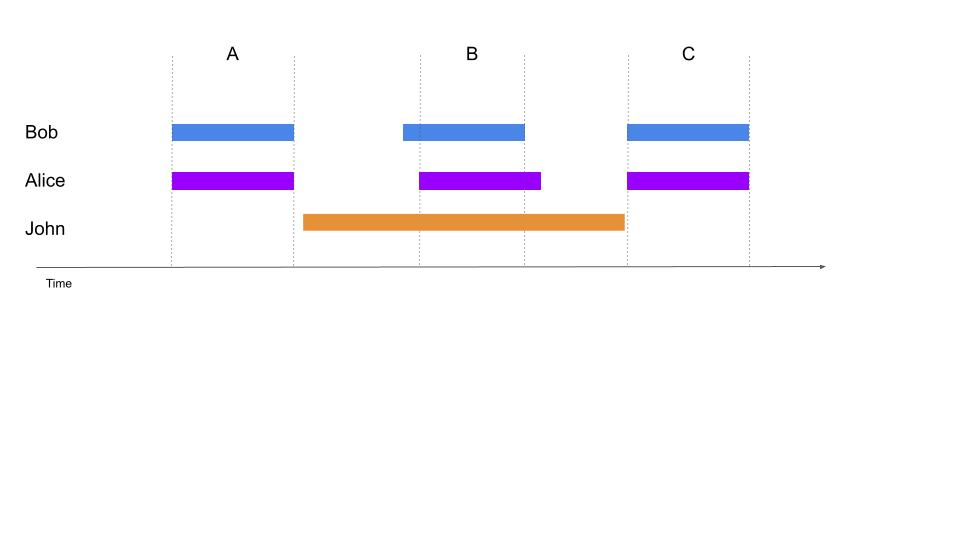
\includegraphics[width=0.8\textwidth]{Fig5a.jpg}
  \label{Annotation:1}%

%\subfloat[]{%
%\centering
%  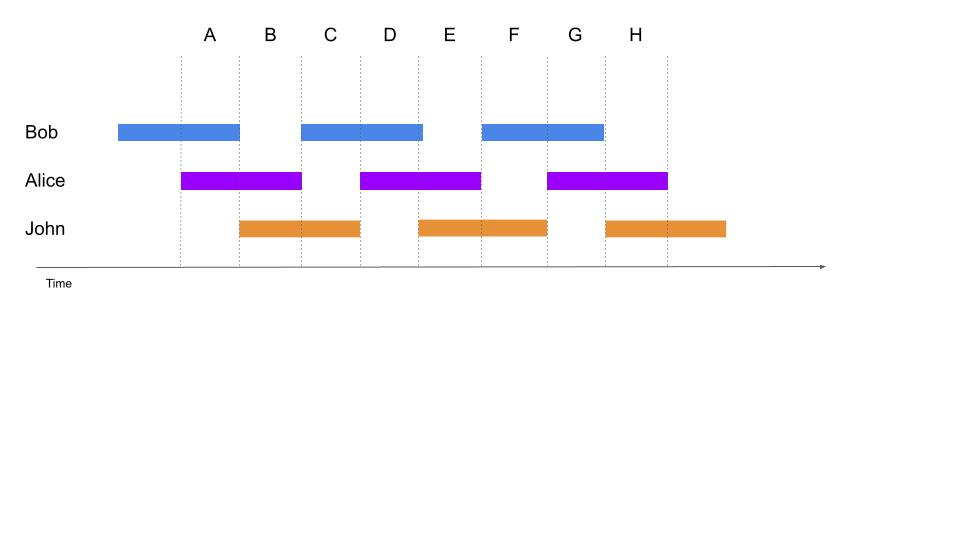
\includegraphics[trim=0 250 25 25, clip, width=0.98\textwidth]{Fig3b.jpg}
%  \label{Annotation:2}%
%}

\caption{\label{fig:Annotation}\textbf{Example of time-intervals of a recording covered by three annotators}. Automated annotations usually cover whole recordings, while human annotators typically annotate periodic or targeted clips. }

\end{figure*}

In psychometrics, the reliability of annotators is usually evaluated using inter-coder agreement indicators. The Python package enables the calculation of some of these measures, including all of the coefficients implemented in the NLTK package \citep{nltk} such as Krippendorff's Alpha \citep{alpha} and Fleiss' Kappa \citep{kappa}. The gamma method by \citet{gamma}, which aims to improve upon previous indicators by evaluating simultaneously the quality of both the segmentation and the categorization of speech, has been included \emph{via} the \texttt{pygamma-agreement} package \citep{pygamma_agreement}.

It should be noted that these measures are most useful in the absence of ground truth, when reliability of the annotations can only be inferred by evaluating their overall agreement. Automatic annotators, however, are usually evaluated against a gold standard produced by human experts. In such cases, the package allows comparisons of pairs of annotators using metrics such as F-score, recall, and precision. Figure \ref{fig:precision} illustrates this functionality. Additionally, the package can compute confusion matrices between two annotators, allowing more informative comparisons, as demonstrated in Figure \ref{fig:confusion}. Finally, the Python package interfaces well with \texttt{pyannote.metrics} \citep{pyannote.metrics}, and all the metrics implemented by the latter can be effectively used on the annotations managed with ChildProject.

\begin{figure*}[htb]

\centering
\includegraphics[width=0.8\textwidth]{Fig6.pdf}

\caption{\label{fig:precision}\textbf{Examples of diarization performance evaluation using recall, precision and F1 score}. Audio from the the public VanDam corpus \citep{vandam-day} is annotated automatically according to who-speaks-when, using: the LENA diarizer; the Voice Type Classifier (VTC) by \citet{lavechin2020opensource}; and manual CHAT transcriptions \citep{MacWhinney2000} adjusted with the Montreal Forced Aligner \citep{mfa} (``cha''). Speech segments are classified among four speaker types: the key child (CHI), other children (OCH), male adults (MAL) and female adults (FEM). Recall, precision and F1 score are calculated for each of these annotations, by comparing them to annotations of 5 $\times$ 1 minute clips annotated by a human annotator using ELAN (``eaf''; \citealt{wittenburg2006elan}). The clips with the most adult words were targeted.
}

\end{figure*}


\begin{figure*}[htb]

\centering
\includegraphics[width=\textwidth]{Fig7.pdf}

\caption{\label{fig:confusion}\textbf{Example of diarization performance evaluation using confusion matrices}
VTC annotations of the public VanDam corpus \citep{vandam-day} are compared to a gold standard manually annotated using ELAN (eaf). The first coefficient of the left side matrix should be read as: ``43\% of CHI segments from the VTC were also labelled as CHI by the human annotator'' (i.e. as the precision of the algorithm). The first coefficient of the right side matrix should be read as: ``95\% of the portions labelled as CHI speech by the annotator were also labelled as CHI by the VTC'' (i.e. as the recall of the algorithm). The sum of each row may exceed one due to overlapping speech. However, the diagonal should ideally be only ones.
}

\end{figure*}


\section{Generalization}

The kinds of problems that our proposed approach addresses are relevant to at least three other bodies of data, all of them based on large datasets collected with wearables. First, there is a line of research on interaction and its effects on well-being among neurotypical adults (e.g., \cite{ear1}). Second, audio data from wearables holds promise for individuals with medical and psychological conditions that have behavioral consequences which can evolve over time, including conditions that lead to coughing \citep{Wu2018} and/or neurogenerative disorders \citep{riad2020vocal}. Third, some researchers hope to gather datasets on child development combining multiple information sources, such as parental reports, as well as other sensors picking up motion and psychophysiological data, with the goal of potentially intervening when it is needed \citep{levin2021sensing}.

Our proposed solution can be readily adapted to the first body of data: All that would need to be changed is renaming children.csv to participants.csv; renaming child\_id to participant\_id; and adapting which columns are mandatory and their format (e.g., it is cumbersome to express age in days for adults).

Generalizing our solution to the second body of data requires more adaptation. For such use cases, it would be ideal for the equipment to be left in the patients' house, so that it can be used for instance one day a week or month. Additional work is needed to facilitate this, ranging from making the equipment easier to use and more robust by for instance facilitating charging and secure data transfer from such off-site locations.

The third use case requires further adaptation, in addition to those just mentioned (making the sensors easy to use and allowing data transfer from potentially insecure home settings). In particular, multiple sensors' data need to be integrated together and time-stamped. We have made some progress in this sense in the context of the collection of multiple audio tracks collected with different physical devices (example forthcoming), but have not yet developed structure and code to support the integration of pictures, videos, heart rate data, parental questionnaire data, etc. 

\section{Limitations}

DataLad and git-annex are well-documented, and, on the user's end, little knowledge beyond that of git is needed. Maintainers and resource administrators, however, will need a certain level of understanding in order to take full advantage of these tools.
Recently, \citet{Powell2021} has emphasized the shortcomings of decentralization and the inconveniences of a proliferation of databases with different access protocols. In the future, sharing data could be made even easier if off-the-shelf solutions compatible with DataLad were made readily available to linguists, psychologists, and developmental scientists. To this effect, we especially call for the attention of our colleagues working on linguistic databases. We are pleased to have found a solution on GIN -- but it is possible that GIN administrators agreed to host our data because there is some potential connection with neuroimaging, whereas they may not be able to justify their use of resources for under-resourced languages and/or other projects that bear little connection to neuroimaging; also, there is no guarantee that the service will last for as long as our corpora may require it.

We should stress again that the use of the ChildProject package does not require the datasets to be managed with DataLad. They do need, however, to follow certain standards. Standards, of course, do not come without their own issues, especially in the present case of a maturing technique. They may be challenged by ever-evolving software, hardware, and practices. However, we believe that the benefits of standardization outweigh its costs provided that it remains reasonably flexible. Such standards will further help to combine efforts from different teams across institutions. More procedures and scripts that solve recurrent tasks can be integrated into the ChildProject package, which might also speed up the development of future tools. 
One could argue that new proposed standards most usually end up increasing the amount of competing standards instead of bringing consensus. Nonetheless, if one were to eventually impose itself, well-structured datasets would still be easier to adapt than disordered data representations. Meanwhile, we look forward to discussing standards collaboratively with other teams via the GitHub platform, where anyone can create issues for improvements or bugs, submit pull-requests to integrate an improvement they have made, and/or have relevant conversations in the forum. Also, it should be emphasized once again that this package does not attempt to enforce specific annotation software or formats, which would be impossible and undesirable, but rather aims at facilitating analyses by incorporating this wide variety of formats into consistent data structures.

Finally, this paper has laid out technical solutions to key issues surrounding long-form recordings, but we have remained silent about how the community can address these while bearing in mind broader ethical issues. For example, speech and language technology has an unfortunate history of focusing on speech and language data over the communities who really own these data \citep{bird2020decolonising}. These ethical and justice issues are crucial and we hope there is more discussion about them in the community using long-form recordings. A case has recently been made about the possibility of building a secure and distributed "World Behavior Bank" \citep{cychosz2021using}, whose governance would include representatives of such populations to make sure that re-use considers potential benefits and harms for participants, participants' families (current and future), as well as more broadly their communities (see also discussions surrounding a Heritage Data Reuse Charter, \url{https://www.dariah.eu/activities/open-science/data-re-use/}).

\section{Summary}

% removed: assessing data reliability
% Data managers should be interested in DataLad because it might benefit to many studies, beyond long-form recordings. We should convince them it is worth diving into it

We provide a solution to the technical challenges related to the management, storage and sharing of datasets of child-centered long-form recordings. This solution relies on four components: i) a set of standards for the structuring of the datasets; ii) \emph{ChildProject}, a Python package to enforce these standards and perform useful operations on the datasets; iii) DataLad, a mature and actively developed version-control software for the management of scientific datasets; and iv) GIN, a storage provider compatible with Datalad. Building upon these standards, we also provide tools to simplify the extraction of information from the annotations and the evaluation of their reliability along with the Python package. The four components of our proposed design serve partially independent goals and can thus be decoupled, but we believe their combination would greatly benefit the technique of long-form recordings applied to language acquisition studies.

\section*{Declarations}

\subsubsection*{Funding} 
This work has benefited from funding and/or institutional support from Agence Nationale de la Recherche (ANR-17-CE28-0007 LangAge,
ANR-16-DATA-0004 ACLEW, ANR-14-CE30-0003 MechELex, ANR-17-EURE-0017);
and the J. S. McDonnell Foundation Understanding Human Cognition Scholar Award. We also benefited from code developed in the Bridges system, which is
supported by NSF award number ACI-1445606, at the Pittsburgh
Supercomputing Center (PSC), using the Extreme Science and Engineering Discovery Environment
(XSEDE), which is supported by National Science Foundation grant number OCI-1053575. Additionally, we benefited from processing in GENCI-IDRIS, France (Grant-A0071011046). Some capabilities of our software depend on  the Zooniverse.org platform, the development of which is funded by generous support, including a Global Impact Award from Google, and by a grant from the Alfred P. Sloan Foundation. The funders had no impact on this study.

\subsubsection*{Conflicts of interest/Competing interests}

The authors have no conflict of interests to disclose.

\subsubsection*{Availability of data and material}

This paper does not directly rely on specific data or material.

\subsubsection*{Code availability}

The present paper can be reproduced from its source, which is hosted on GIN at \url{https://gin.g-node.org/LAAC-LSCP/managing-storing-sharing-paper}.
The ChildProject package is available on GitHub at \url{https://github.com/LAAC-LSCP/ChildProject}. 
A step-by-step tutorial to launch annotation campaigns on Zooniverse is published along with the source code at \url{https://doi.gin.g-node.org/10.12751/g-node.k2h9az} \citep{zooniverse_example}.
We provide scripts and templates for DataLad managed datasets at \url{http://doi.org/10.17605/OSF.IO/6VCXK} \citep{datalad_procedures}. We also provide a DataLad extension to extract metadata from corpora of long-form recordings \citep{datalad_extension}.

\appendix

\section{Examples of storage strategies}\label{appendix:examples}

\subsection{\label{sec:example1}Example 1 - sharing a dataset within the lab}

In the first example, Alice is hosting large datasets of a few terabytes of recordings and annotations and she wants to share them with Bob - a collaborator from her own institution - in a secure manner. Alice and Bob are familiar with GitHub, and they like its user-friendly features such as issues and pull requests. However, GitHub cannot handle such amounts of data.

Alice decides to store the git repository itself on GitHub -- or a GitLab instance, it would not matter -- thus allowing to benefit from their nice features while hosting the large files -- the recordings and annotations -- elsewhere. Alice's laboratory has its own cluster, with a large storage capacity. Thus, she decides to host the files there for free rather than using a Cloud provider.

Since Bob has been given SSH access to the cluster and belongs to the right UNIX group, he can download recordings and annotations from their joint institution cluster. Alice also made sure to configure the dataset in a way that makes sure every change published to GitHub is also published to the cluster, with DataLad's ``publish-depends'' option. 

For backup purposes, a third sibling is hosted on Amazon S3 Glacier -- which is cheaper than S3 at the expense of higher retrieval costs and delays -- as a git-annex \href{https://git-annex.branchable.com/special_remotes/}{special remote}\footnote{\url{https://git-annex.branchable.com/special_remotes/}}. Special remotes do not store the git history and they cannot be used to clone the dataset. However, they can be used as a storage support for the recordings and other large files. In order to increase the security of the data, Alice uses encryption. Git-annex implements several encryption schemes\footnote{\url{https://git-annex.branchable.com/encryption/}}. The hybrid scheme allows to add public GPG keys at any time without additional decryption/encryption steps. Each user can then later decrypt the data with their own private key. This way, as long as at least one private GPG key has not been lost, data are still recoverable. This is especially valuable in that in naturally ensures redundancy of the decryption keys, which is critical in the case of encrypted backups.

By default, file names are hashed with an HMAC algorithm, and their content is encrypted with AES-128 -- GPG's default --, although another algorithm could be selected.

This setup ensures redundancy of git files (hosted on both GitHub and the cluster) as well as large files (stored on both the cluster and Amazon Deep Glacier). It also allows Bob to signal and correct errors he finds, and/or to add annotations in a straightforward manner, benefiting Alice. By virtue of having siblings, they can make sure that their local dataset is organized in an identical manner, facilitating collaboration and reproducibility in their analyses.

Table \ref{table:storage1} illustrates such a strategy. In this example, users install the dataset from a private GitHub repository. Continuous testing is configured with Travis CI\footnote{https://travis-ci.com/}, in order to ensure the integrity of the dataset at every step. GitHub Actions could also be used for that purpose\footnote{https://docs.github.com/en/actions}.

We used this strategy -- minus the Glacier backups -- to maintain and deliver 4 datasets with 8700 hours of audio\footnote{\url{https://github.com/LAAC-LSCP/datasets}} for several months. The associated scripts can be found on \cite{datalad_procedures}. We have now transitioned to using GIN for our main site, with our cluster as the backup. The scripts associated to this set-up can be found at the same location.


\begin{table*}[!htbp]
\centering
\begin{tabular}{@{}lllllll@{}}
\toprule
\textbf{Sibling} & \textbf{Provider} & \textbf{Content} & \textbf{Access} & \textbf{Encryption} \\ \midrule
origin   & GitHub     & metadata; scripts & Lab & No  \\
cluster  & SSH server & everything & Lab & No  \\
backup & Amazon Deep Glacier  &  recordings; annotations  & Lab            & AES-128 \\ \bottomrule
\end{tabular}
\caption{\label{table:storage1}Example 1 - Storage strategy example relying on GitHub and a cluster to deliver the data.}
\end{table*}

\subsection{Example 2 - sharing large datasets with outside collaborators (S3)}

The previous strategy is not suitable when complex permissions are required, since SSH remotes only handle Unix-style permissions (user, group, all).

Moreover, Alice may want to share the dataset with collaborators outside her lab, without giving them SSH access to its cluster. Or, she may not even own the infrastructure that would allow her to store and share such large amounts of data. 

Instead, she decides to use Amazon S3 together with GitHub. Authorized users are provided their own Amazon S3 API key and secret, which are managed with Amazon's Identity and Access Manager (IAM). The GitHub is stripped from all confidential data, which are stored in the S3 annex only, allowing to manage access permissions entirely through IAM. This strategy is used by the Human Connectome Project\footnoteref{note:hcp}.

Furthermore, Alice makes sure to encrypt GDPR relevant data, using strong symmetric encryption (AES-128). This strategy is illustrated in Table \ref{table:storage2}.

\begin{table*}[!htbp]
\centering
\begin{tabular}{@{}lllllll@{}}
\toprule
\textbf{Sibling} & \textbf{Provider} & \textbf{Content} & \textbf{Access} & \textbf{Encryption} \\ \midrule
origin   & GitHub     & metadata; scripts & Collaborators & No  \\
s3 & Amazon S3  &  recordings; annotations  & Collaborators  & AES-128 \\ \bottomrule
\end{tabular}
\caption{\label{table:storage2}Example 2 - Storage strategy example relying on GitHub and Amazon S3.}
\end{table*}

Amazon is superior to most alternatives for a number of reasons, including that it is highly tested, developed by engineers with a high-level of knowledge of the platform, and widely used. This means that the code is robust even before it is released, and it is widely tested once it is released. The fact that there are many users also entails that issues or questions can be looked up online. In addition, in the context of data durability, Amazon is a good choice because it is ``too big to fail'', and thus probably available for the long-term. Moreover, in sheer terms of flexibility and coverage, Amazon provides a whole suite of tools (for data sharing, backups, and processing), which may be useful for researchers with little access to high-capacity infrastructures. Additionally, it is not very costly (see comparison table on \url{https://childproject.readthedocs.io/en/paper/vandam.html?highlight=amazon#where-to-publish-my-dataset}).

\subsection{Example 3 - sharing large datasets with outside collaborators  and multi-tier access (GIN)}\label{appendix:gin}

Due to legislation in some countries, there are researchers who may not be authorized to store their data on Amazon. If they also do not have access to a local cluster (see Example 1) and/or even in the case that they have a local cluster, but need finer control of access permissions, there are alternatives which can be used as a workaround.

Finding herself in this setting, Alice decides to use the G-Node Infrastructure (GIN)\footnote{\url{https://gin.g-node.org/}}, which is dedicated to providing ``Modern Research Data Management for Neuroscience''. GIN is similar to GitLab and GitHub in many aspects, except that it also supports git-annex and thus can directly host the large files that required third-party providers while using those platforms.

Just like GitLab or GitHub, it can handle complex permissions, at the user or group-level, thus surpassing Unix-style permissions management.

In this case, Alice needs three permission tiers: 1) read-only access to anonymized data, 2) read-only access to confidential data, and 3) read and write access to the whole data. In order to achieve this, she creates two GIN siblings per dataset: \texttt{origin} and \texttt{confidential}. The dataset is configured to publish all the files whose path contains \path{/confidential/} to the \path{confidential} repository, while the rest of the data is published to \texttt{origin}. Alice could then great read-only access to \texttt{origin} to both Bob and Carol, while restricting the access to \texttt{confidential} to Bob only.

Since Alice has not been allowed to use a cloud provider, and is lacking a local infrastructure, she needs an alternate solution for her backups. She may use external hard drives, as DataLad allows to push data to a local storage as with any other kind of storage.

Table \ref{table:storage3} sums up this strategy, which is currently used to deliver the EL1000 dataset\footnote{\url{https://gin.g-node.org/EL1000/EL1000}} -- except for the backup, which is located at our cluster --. The EL1000 is a composite dataset, created by the contribution of 18 different teams that collected data independently but using comparable methods.

\begin{table*}[!htbp]
\centering
\begin{tabular}{@{}lllllll@{}}
\toprule
\textbf{Sibling} & \textbf{Provider} & \textbf{Content} & \textbf{Access} & \textbf{Encryption} \\ \midrule
origin   & GIN     & files NOT matching \path{**/confidential/*} & \begin{tabular}[t]{@{}l@{}}Alice (read+write);\\Bob, Carol (read-only)\end{tabular} & No  \\
confidential & GIN  & files matching \path{**/confidential/*}  & \begin{tabular}[t]{@{}l@{}}Alice (read+write);\\Bob (read-only)\end{tabular}  & No \\ 
backup & \begin{tabular}[t]{@{}l@{}}external\\hard drive\end{tabular}  & everything  & Alice  & No \\\bottomrule
\end{tabular}
\caption{\label{table:storage3}Example 3 - Storage strategy example relying solely on GIN to deliver the data.}
\end{table*}


\subsection{Example 4 - Sharing smaller datasets (OSF)}


The Open Science Framework (OSF) is especially interesting because it supports DOI registration, providing permanent URLs to access the datasets. Moreover, an extension of DataLad has specifically been developed to work with OSF, which may host both the git repository and the large files (see Table \ref{table:providers}). In addition, Shibboleth credentials can be used with OSF.

Low quotas are an important downside with OSF. Public projects are limited to 50 GB, and private projects cannot exceed 5 GB, which is too low for most long-form datasets.
However, OSF could be used only to host the git repository, effectively providing a permanent URL from which the dataset can be installed, as long as the content of the large files remains available from a third-party provider, e.g. with Amazon S3. Table \ref{table:storage4} illustrates such a strategy.

\begin{table*}[!htbp]
\centering
\begin{tabular}{@{}lllllll@{}}
\toprule
\textbf{Sibling} & \textbf{Provider} & \textbf{Content} & \textbf{Access} & \textbf{Encryption} \\ \midrule
origin   & OSF     & metadata; scripts & Everyone & No  \\
s3 & Amazon S3  & annotations; recordings & Alice, Bob and Carol  & No \\ \bottomrule
\end{tabular}
\caption{\label{table:storage4}Example 4 - Storage strategy example relying on OSF and Amazon S3 to deliver the data.}
\end{table*}

We use a reversed approach for our demo dataset\footnote{\url{https://github.com/LAAC-LSCP/vandam-daylong-demo}} based on  \citep{vandam-day}, by hosting the git repository on GitHub, and hosting the large files on OSF. This is possible only because of the small size of the dataset.

\bibliographystyle{spbasic}
\bibliography{references}

\end{document}
